Some general instructions on using the template follow.
It is a good idea to keep this file around for future reference.


\subsection{Structure}
\label{sec:instructions:structure}
\lipsum[6] % Dummy text

\paragraph{Paragraph Description} \lipsum[7] % Dummy text

\paragraph{Different Paragraph Description} \lipsum[8] % Dummy text


\subsection{Citations and References}
\label{sec:instructions:references}
A statement requiring citation \cite{Figueredo:2009dg}.


\subsection{Figures}
\label{sec:instructions:figures}

Reference to \autoref{fig:gallery}.

\begin{figure}[tb]
\centering
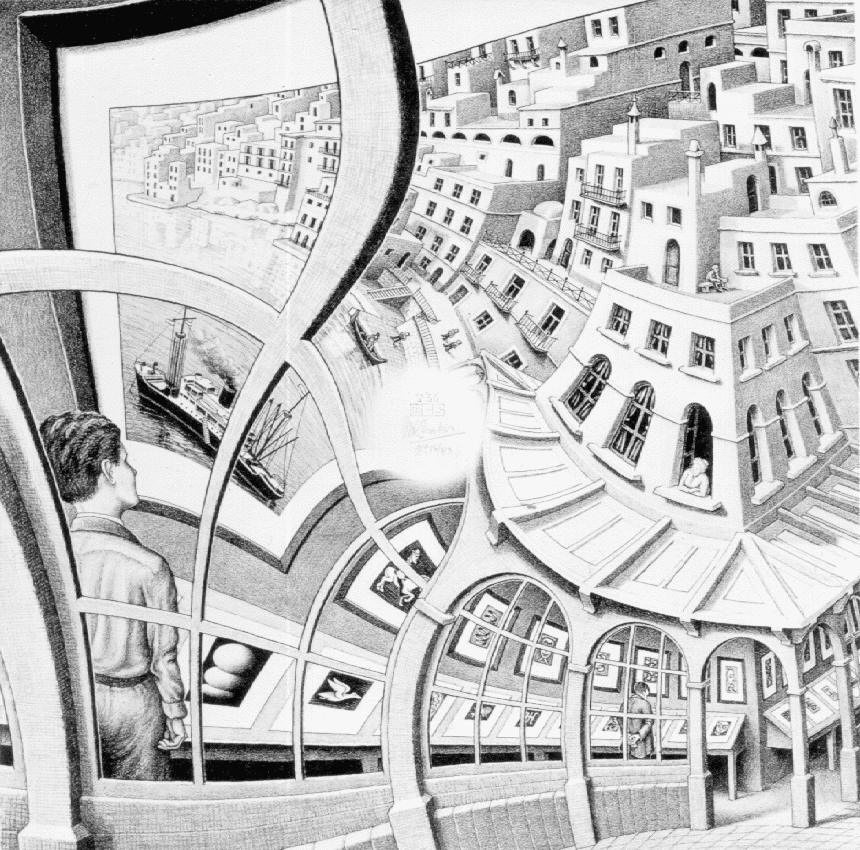
\includegraphics[width=0.5\columnwidth]{GalleriaStampe}
% The text in the square bracket is the caption for the list of figures while the text in the curly brackets is the figure caption
\caption[An example of a floating figure]{
  An example of a floating figure (a reproduction from the
  \emph{Gallery of prints}, M.~Escher,\index{Escher, M.~C.}
  from \url{http://www.mcescher.com/}).
}
\label{fig:gallery}
\end{figure}

Reference the figure composed of multiple subfigures as \autoref{fig:esempio}.
For sub-figures, reference as \autoref{fig:ipsum}.
You can also reference as \figureautorefname~\vref{fig:ipsum},
which will also add the page number where appropriate.

\lipsum[15-18] % Dummy text

\begin{figure}[tb]
\centering
\subfloat[A city market.]{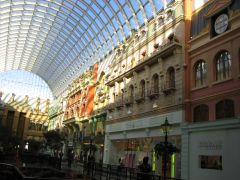
\includegraphics[width=.45\columnwidth]{Lorem}} \quad
\subfloat[Forest landscape.]{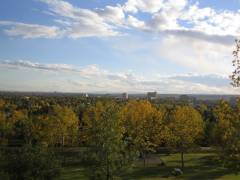
\includegraphics[width=.45\columnwidth]{Ipsum}\label{fig:ipsum}} \\
\subfloat[Mountain landscape.]{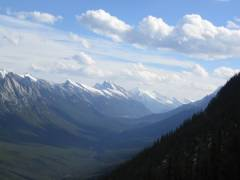
\includegraphics[width=.45\columnwidth]{Dolor}} \quad
\subfloat[A tile decoration.]{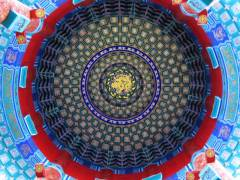
\includegraphics[width=.45\columnwidth]{Sit}}
\caption[A number of pictures.]{A number of pictures with no common theme.} % The text in the square bracket is the caption for the list of figures while the text in the curly brackets is the figure caption
\label{fig:esempio}
\end{figure}

\subsection{Comments and to-do's}
There are many ways to add to-do items.
You can use \TODO{XX}{number here} to put a note with a side-note comment.

To add a reminder to add a reference to a future section use
\todoref{Section on benefits}.



\subsection{Math}

Some mathematics in the text: $\cos\pi=-1$ and $\alpha$.

\begin{equation}
\cos^3 \theta =\frac{1}{4}\cos\theta+\frac{3}{4}\cos 3\theta
\label{eq:refname2}
\end{equation}

\lipsum[5] % Dummy text

\begin{definition}[Gauss]
To a mathematician it is obvious that
$\int_{-\infty}^{+\infty}
e^{-x^2}\,dx=\sqrt{\pi}$.
\end{definition}

\begin{theorem}[Pythagoras]
The square of the hypotenuse (the side opposite the right angle) is equal to the sum of the squares of the other two sides.
\end{theorem}

\begin{proof}
We have that $\log(1)^2 = 2\log(1)$.
But we also have that $\log(-1)^2=\log(1)=0$.
Then $2\log(-1)=0$, from which the proof.
\end{proof}

\subsection{Methods}

\lipsum[5] % Dummy text

\begin{enumerate}[noitemsep] % [noitemsep] removes whitespace between the items for a compact look
\item First item in a list
\item Second item in a list
\item Third item in a list
\end{enumerate}

%------------------------------------------------

\subsection{Subsection}

\lipsum[11] % Dummy text

\subsubsection{Subsubsection}

\lipsum[12] % Dummy text

\begin{description}
\item[Word] Definition
\item[Concept] Explanation
\item[Idea] Text
\end{description}

\lipsum[12] % Dummy text

\begin{itemize}[noitemsep] % [noitemsep] removes whitespace between the items for a compact look
\item First item in a list
\item Second item in a list
\item Third item in a list
\end{itemize}

\subsubsection{Table}

\lipsum[13] % Dummy text

\begin{table}[hbt]
\caption{Table of Grades}
\centering
\begin{tabular}{llr}
\toprule
\multicolumn{2}{c}{Name} \\
\cmidrule(r){1-2}
First name & Last Name & Grade \\
\midrule
John & Doe & $7.5$ \\
Richard & Miles & $2$ \\
\bottomrule
\end{tabular}
\label{tab:label}
\end{table}

Reference to Table~\vref{tab:label}. % The \vref command specifies the location of the reference




%%% Local Variables:
%%% mode: latex
%%% TeX-master: "{{cookiecutter.file_name}}"
%%% End:
